\begin{tcolorbox}[colback=white,colframe=black,opacityframe=0,colbacktitle=black,title={\textbf{Problem 5 [\examproblemweight\ points]}}]
\begin{enumerate}[label=(\alph*)]
	\item Consider the function $h(x) = 3-(x+1)^2$.
	\begin{enumerate}[label=(\roman*)]
		\item \textbf{(2 points)} Identify the zeros of $h$. Give both \textbf{exact} and \textbf{rounded answers to the nearest hundredth} for this part.
		\item \textbf{(4 points)} Observe that $h$ is the result of a combination of transformations on the squaring function $q(x)=x^2$. Identify the transformations used to transform the squaring function $q$ into the function $h$ (for instance, write down ``Dilate horizontally by a factor of $\f13$" if that is a relevant transformation involved to make $h$). 
		
		Then, use those transformations to graph $y=h(x)$ in the Cartesian plane below as accurately as possible. (It is okay to check if your sketch is correct using your graphing calculator for this part!)
	\end{enumerate}
	\hspace*{17em}
	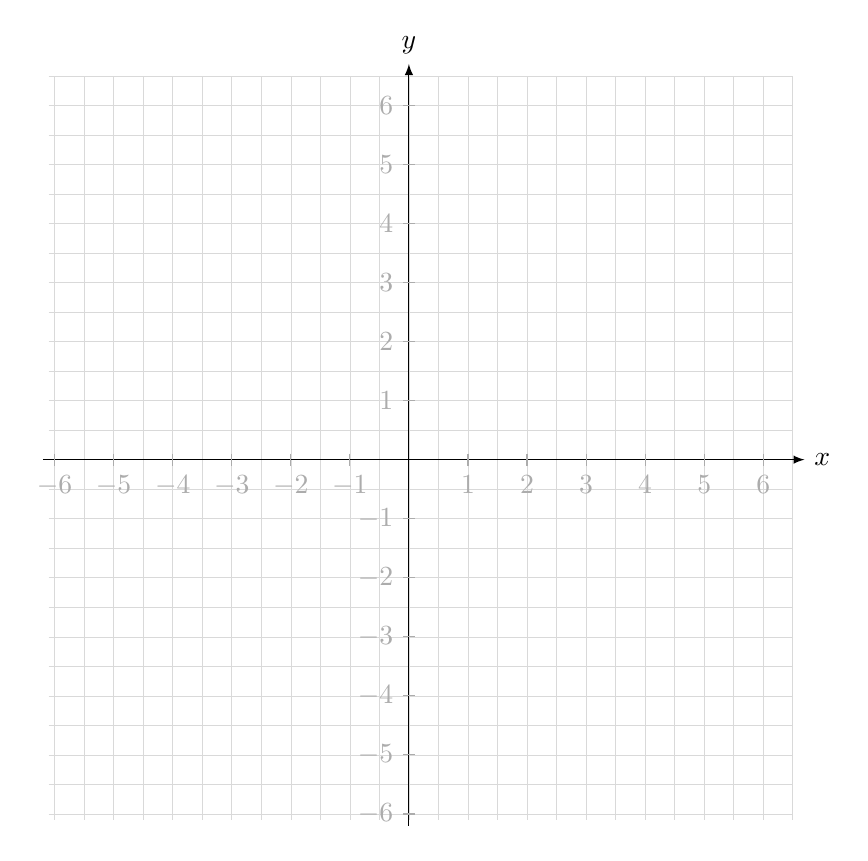
\begin{tikzpicture}[scale=0.75]
		\draw[very thin,color=black!15,step=.5] (-6.1,-6.1) grid (6.5,6.5);
		\draw[-latex] (-6.2,0) -- (6.7,0) node[right] {$x$};
		\draw[-latex] (0,-6.2) -- (0,6.7) node[above] {$y$};
		\foreach \i in {-6,...,-2,-1,1,2,...,6}
		\draw[gray!65] (\i,.1)--(\i,-.1) node[below] {$\i$};
		\foreach \i in {-6,...,-2,-1,1,2,...,6}
		\draw[gray!65] (.1,\i)--(-.1,\i) node[left] {$\i$};
	\end{tikzpicture}
	\item Let $f(x) = \sqrt{3-x}$ and $g(x)=(x+1)^2$.
	\begin{enumerate}[label=(\roman*)]
		\item \textbf{(2 points)} What is the domain of $f+g$?
		\item \textbf{(1 point)} Compute the composition $(f\circ g)(x)$. (You do not need to expand anything, like products of binomials, in your final answer.)
		\item \textbf{(1 point)} What is the domain of $f\circ g$? (Hint: You'll need your graph of $h$ and its zeros from part (a). For what input values of $h$ is the graph at or above the $x$-axis? That should tell you about $\text{domain}(f\circ g)$. Be sure to use \textbf{exact numbers} for the endpoints of your domain intervals.)
	\end{enumerate}
\end{enumerate}
\end{tcolorbox}

\newpage
\noindent \centering Blank page \thepage~for additional work
\newpage
